% =====================================================================
% 6. Area 3 in code: ECG-GPT and LSTM generators (T23, own block)
% =====================================================================
\section{Area 3: autoregressive generators in code (own block)}\label{sec:generative-code}

\subsection{From signal to tokens}

PTB-XL stores every sample as an integer number of microvolts (the code checks it on the training data:
a share \generativeFracOffUvGridTrain{} of the values is off the grid), so the tokenizer
(Listing~\ref{lst:tok}) is exact inside its range. A value in millivolts becomes an integer number of
microvolts, its token is the floor division by the level width $\Delta$ after subtracting the lower end of
the range, and values outside go to the first or last token. The range is 2.56\,mV wide, from
\generativeRangeLoUv{} to \generativeRangeHiUv{}\,\textmu V, centred on training quantiles of lead II.

\lstinputlisting[firstnumber=69,caption={Tokenizer on the microvolt grid (\texttt{src/generative.py},
lines 69--74).},label={lst:tok}]{common/code/tokenizer.py}

Training items are windows of $L+1$ samples starting at a random position of a training record: the
first $L$ tokens are the input and the same tokens shifted by one are the target (teacher forcing). The
window start is drawn from a NumPy generator seeded with the run's seed, which is reproducible because
data loading runs in the main process. An epoch shows every training record once through one random
window. Validation uses fixed windows that together cover every target of every record.

\subsection{Model and loss}

The ECG-GPT reuses Mar\'ia's Transformer blocks with \texttt{causal=True}. The mask is a lower-triangular
boolean matrix, and masked scores are set to $-\infty$ before the softmax, so their weights are exactly
zero (Listing~\ref{lst:causal}; a test checks that the attention maps are lower-triangular and that
changing a future token does not change past outputs).

\lstinputlisting[firstnumber=29,caption={Causal mask and scaled dot-product attention
(\texttt{src/models/attention.py}, lines 29--62).},label={lst:causal}]{common/code/causal_attention.py}

\begin{itemize}[leftmargin=1.2em,itemsep=1pt]
  \item \textbf{Embeddings.} \texttt{nn.Embedding(V, 128)} gives one learned vector per level, as one
        vector per character in the course's text-generation notebooks. The sinusoidal positional encoding
        is a non-persistent buffer: it moves to the GPU with the model, is not trained and is not stored in
        the checkpoint.
  \item \textbf{Cross-entropy over sequences.} Logits $(B, T, V)$ are reshaped to $(B\cdot T, V)$ and
        targets to $(B\cdot T)$ before \texttt{F.cross\_entropy}; otherwise PyTorch would read $T$ as the
        class axis. No softmax in the model: the loss contains it.
  \item \textbf{Per-position cost.} \texttt{log\_softmax} followed by \texttt{gather} gives the
        cross-entropy of every position separately, which the mean loss hides; it is the curve of
        prediction cost against context shown in the PRDL-DL report.
  \item \textbf{Same size for a fair comparison.} The LSTM's hidden size was chosen so that it has about
        the same number of parameters as the ECG-GPT (\generativeParamsLstm{} against
        \generativeParamsBase{}).
\end{itemize}

\subsection{Generation}

Generation slides a window of $L$ tokens one sample at a time: the model predicts the next token from
the last $L$, the token is appended and the window moves. Both models use the same sliding window (the
LSTM state is not carried beyond $L$ samples, which it never saw in training). Only the last position
goes through the output layer. Listing~\ref{lst:sample} shows the sampling rule, following the course
notebook \cite{course_nb_sampling}.

\lstinputlisting[firstnumber=468,caption={Greedy, temperature and top-$k$ sampling
(\texttt{src/generative.py}, lines 468--485).},label={lst:sample}]{common/code/sample_next.py}

\begin{itemize}[leftmargin=1.2em,itemsep=1pt]
  \item \textbf{Reproducible sampling.} \texttt{torch.multinomial} draws with a \texttt{torch.Generator}
        seeded once per model, under \texttt{model.eval()} and \texttt{torch.no\_grad()}.
  \item \textbf{Memory grows with $L^2$.} Generating 64 windows of 500 tokens ran out of memory on the
        4\,GB GPU (Appendix~\ref{app:ai-code}, Sheet C1); generation batches now shrink as $(250/L)^2$ for
        longer contexts and the GPU is freed between models.
  \item \textbf{Cost.} The median epoch takes \generativeEpochTimeMedianBase{}\,s for the ECG-GPT
        baseline, \generativeEpochTimeMedianLstm{}\,s for the LSTM and \generativeEpochTimeMedianCtxFiveZeroZero{}\,s
        with a 5\,s context; the 24 runs took several hours of training, and almost all of them used the
        whole 50-epoch budget.
\end{itemize}

% Shared float (common/make_floats.py). Figure: figures/generative_curves.pdf
\begin{figure}[htbp]
\centering
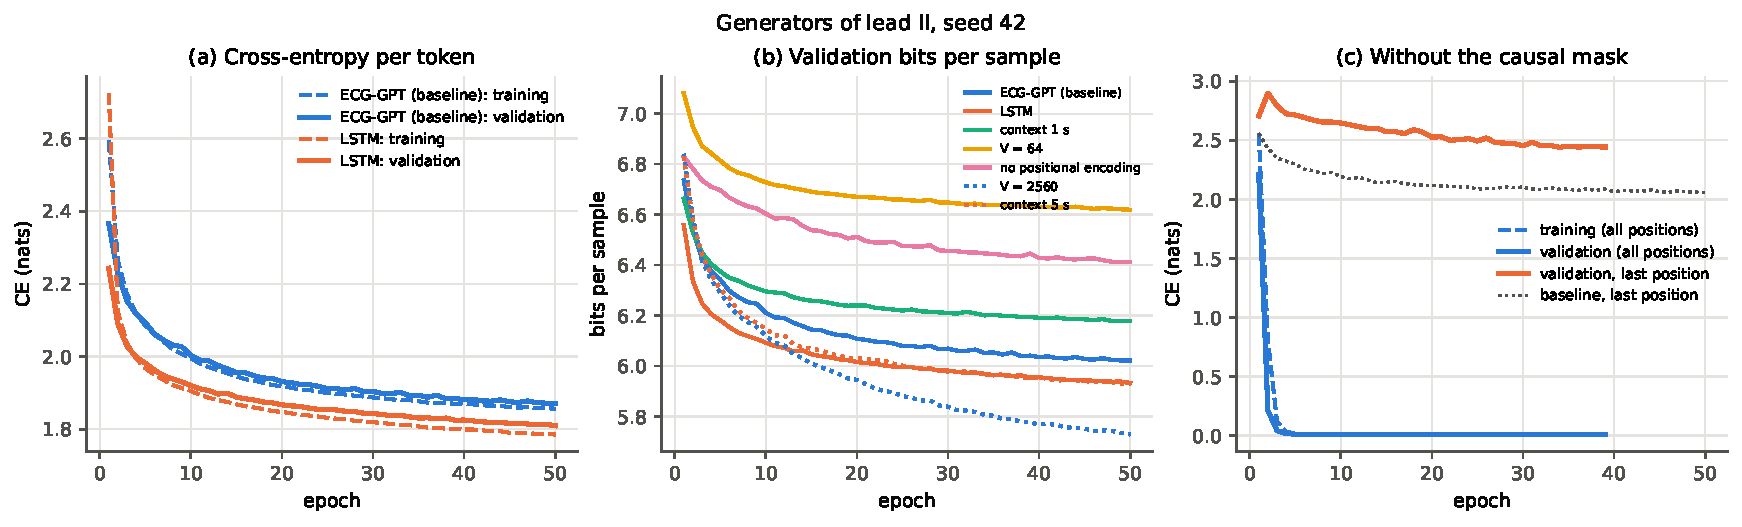
\includegraphics[width=\textwidth,height=0.42\textheight,keepaspectratio]{figures/generative_curves.pdf}
\caption[Generators: learning curves]{Generators of lead II, seed 42. (a) Cross-entropy per token of the ECG-GPT baseline and the LSTM. (b) Validation bits per sample of every configuration. (c) The ECG-GPT without the causal mask: training and validation cross-entropy over all positions and at the last position, with the baseline's last position for reference.}
\label{fig:generative_curves}
\end{figure}

% Shared float (common/make_floats.py). Figure: figures/generative_sampling.pdf
\begin{figure}[htbp]
\centering
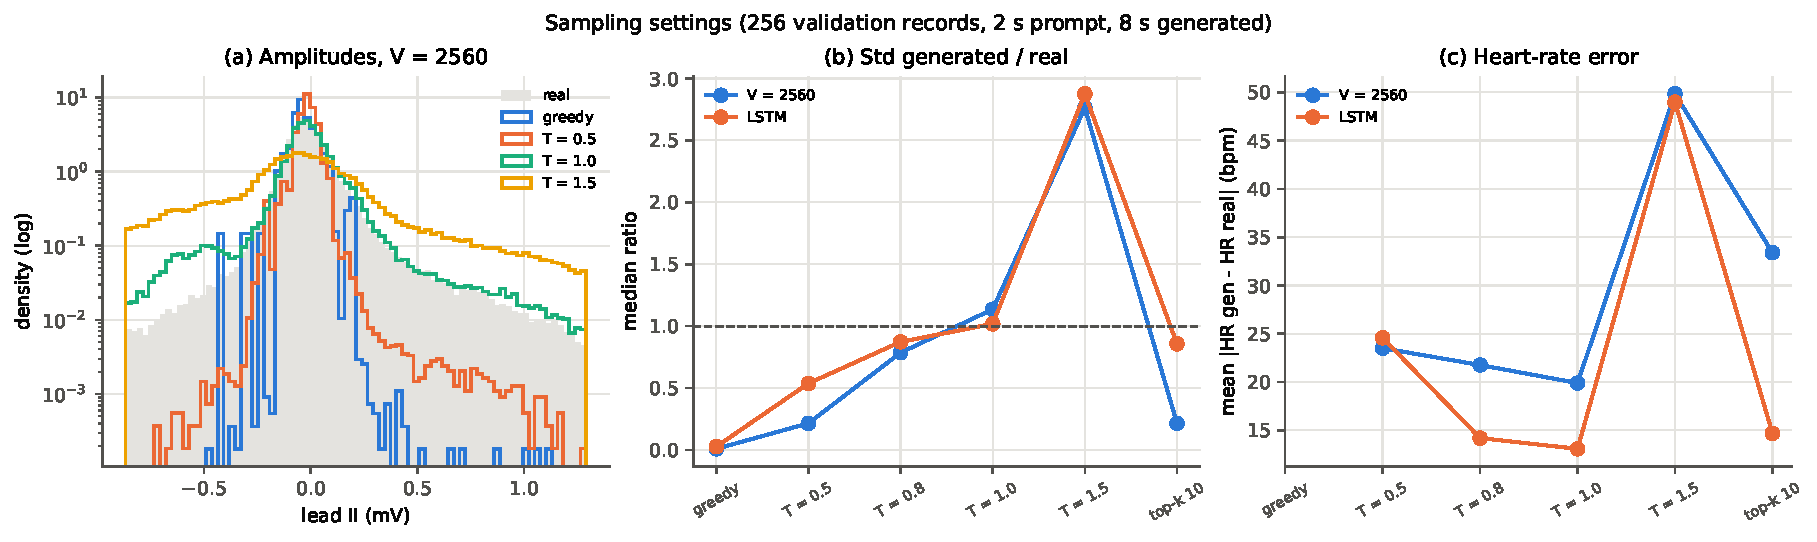
\includegraphics[width=\textwidth,height=0.42\textheight,keepaspectratio]{figures/generative_sampling.pdf}
\caption[Generators: sampling settings]{Sampling settings (256 validation records, 2\,s prompt, 8\,s generated). (a) Amplitude distributions of the generated signals against the real ones ($V = 2560$). (b) Median ratio of generated to real standard deviation. (c) Mean absolute heart-rate error.}
\label{fig:generative_sampling}
\end{figure}


\subsection{Evaluation code}

Besides cross-entropy and perplexity (exponential of the mean cross-entropy per token over the whole
split, not averaged per batch), the block computes bits per sample, unigram and bigram counting
baselines with add-one smoothing for each vocabulary, the ``next sample = this sample'' error, and, for
generated signals, the standard-deviation ratio, the share of flat records, the Wasserstein distance
between amplitude distributions and a heart rate from R peaks (local maxima above a threshold taken
from the real prompt, at least 0.3\,s apart). The heart-rate rule is simple and not a validated
detector; it finds a rate in a share \generativeRealHrDefinedFrac{} of the real continuations.
